\chapter{Motor Learning in Virtual Reality}
\label{chapter:theoretical_background}
The aquisition and improvement of movements is called motor learning~\cite{mlbook}. 

\section{Mixed Reality}
\label{section:mixed_reality}
Milgram and Kishinho~\cite{mrcontinuum} describe Mixed Reality for visual displays on a continuum (see seminar thesis chapter 2.3). In Virtual Reality the environment is blocked completely while in Augmented Reality the environment is visible and augmented with digital elements. During Motor Learning the visual perception of the own body is desireable, though the approach of augmenting the real-world body with a virtual guidance visualisation is promising. But todays AR-technology provide a small field of view. A solution to this could be the video see-through technology, but this is also limited by latency and distrotion.\\
The perception of the own body can also be achieved by rendering the body of the learner and though can be established in VR. This solution is applied in the proposed study design and the study takes place in Virtual Reality.

\section{Motor Learning}
\label{section:motor_learning}
Motor Learning is achieved through instruction, trying, imitation or a combination of them. The process of Motor Learning can be divided into three parts: cognitive stage, assosiative stage and autonomous stage. In the cognitive stage, training methods are most efficient and the performance gain ist the highest among the stages~\cite{mlbook}. Tasks that belong to this stage are thereby best suited for a study. A detailed description of the stages can be found in the preceeding seminar thesis.\\
Movements can be calassified by two means: by the particular movements  and based on the perceptual attributes. Based on the particular movements, the classification is described by a continuum, compare figure~\ref{fig:movement_classification1}. On the extremes of the continuum are discrete movements and continuous movements. Between these extremes, serial movements are located. For a detailed description please refere to seminar thesis chapter 2.2. Discrete movements are too short for an evaluation. Continuous movements do not have an recognisable beginning and thereby they are not suitable for the study in question either. Serial movements are basically chained discrete movements with a recognisable beginning and end. This allows to determine a task decomposition compare section \ref{handlingphysicalload} and a evaluation of particular tasks. Discrete movements are widely used for reseach in Motor Learning, for example ~\cite{lightguide,mythaichicoaches,elearningma}, therefore, the study task design is based on discrete movements.\\
The classification based on the perceptual attributes is also represented by an continuum and includes the environment the movement is performed compare figure~\ref{fig:movement_classification2}. At the extremes of the continuum open skills and closed skills are located. For closed skills, the environment is predictable while in open skills the environment is not predictable. The study aims to analyse the learners performance of following a movement and not how the learner can adapt to environmental changes, the task for this study must be located on the left hand side of the continuum: closed skills.
\begin{figure}[htb]
	\centering
	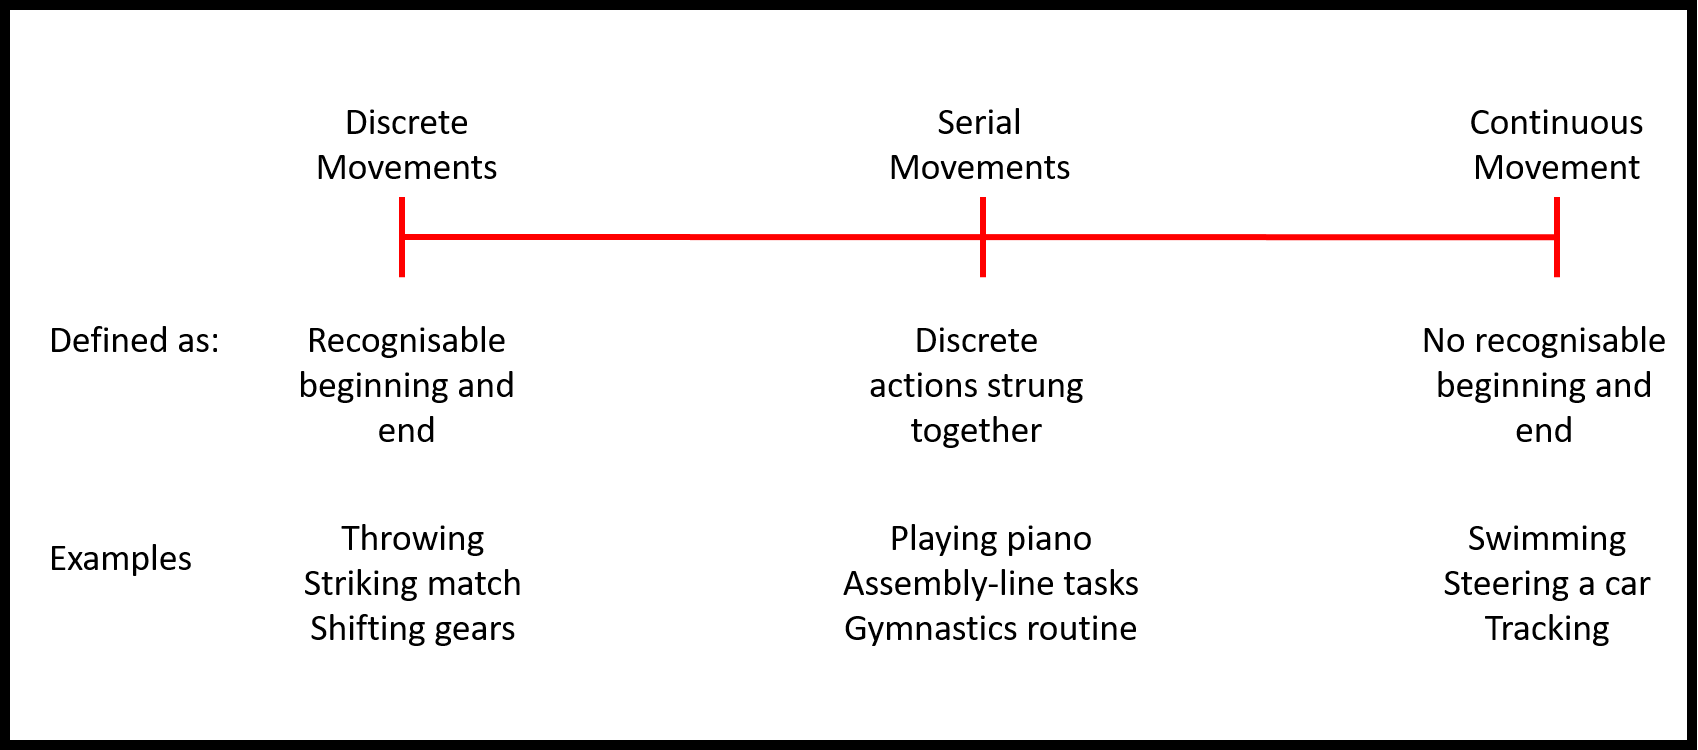
\includegraphics[width=\textwidth]{figures/movement_classification.png}
	\caption[Movement classification 1]{Movement classification 1 \cite{mlbook}}
	\label{fig:movement_classification1}
\end{figure}
\begin{figure}[htb]
	\centering
	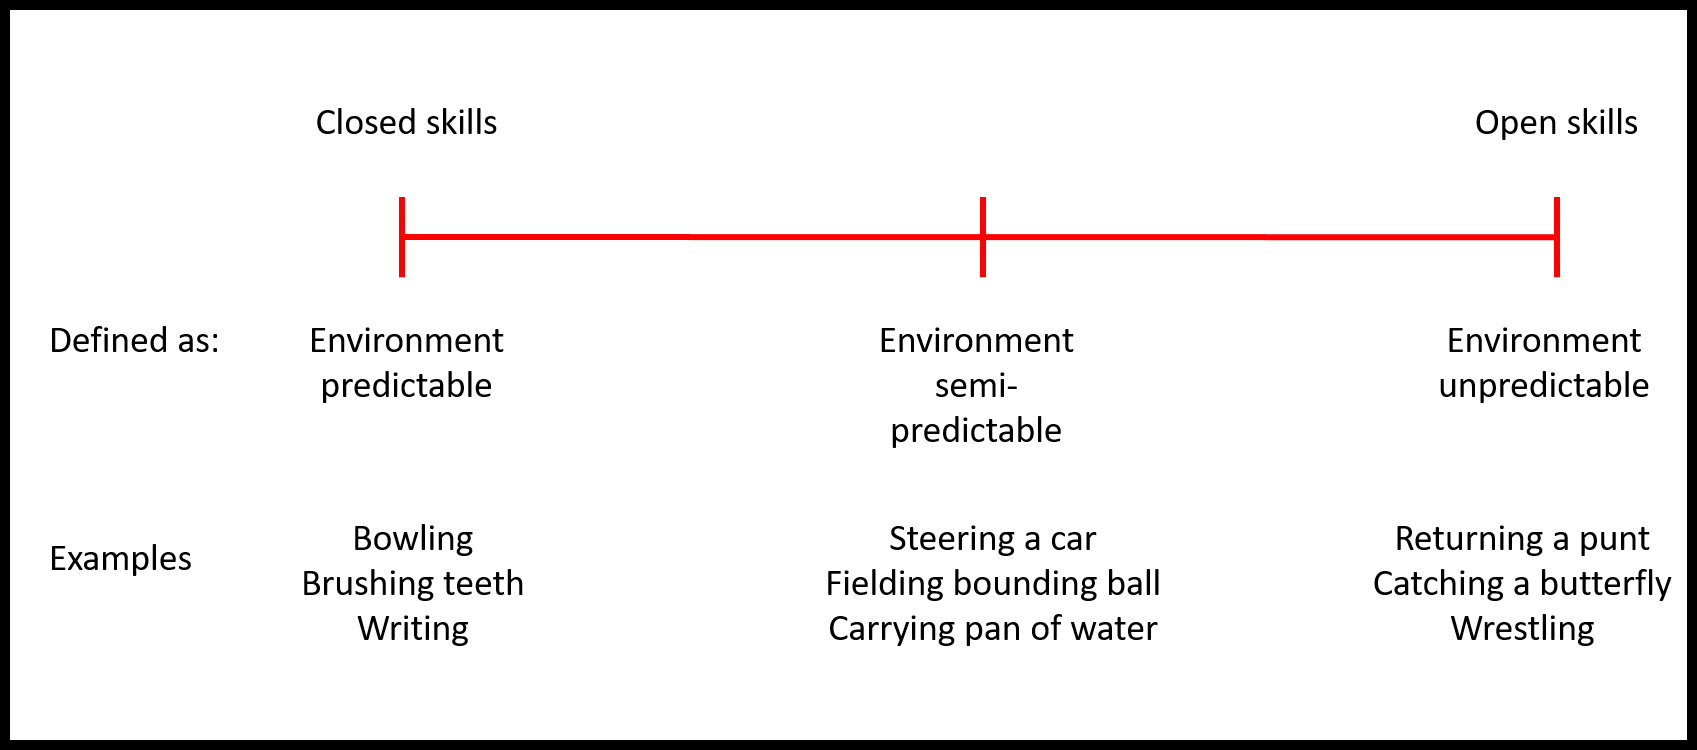
\includegraphics[width=\textwidth]{figures/movement_classification2.png}
	\caption[Movement classification 2]{Movement classification 2 \cite{mlbook}}
	\label{fig:movement_classification2}
\end{figure}

\subsection{Measurements for Motor Learning}
\label{section:measures_for_ml}

\section{Visual Perspectives}
\label{section:visual_perspectives}
Wang and Milgram~\cite{centricitycontinuum} describe visual perspectives by the centricity continuum~\ref{fig:ego-exo-continuum}. On the left extreme on the continuum, the ego-centric visual perspective is located, on the right extreme the exo-centric visual perspective can be found, while the middle part represents tethered visual perspectives. By moving from the left to the right the so called tethering distance increases. The tethering distance describe the distance of the anchor point of the eyes to the object to control. In this work the object to control is the learners avatar guidance visualisation. Furthermore, Wang and Milgram distinguish tethered visual perspective in dynamic and rigid, a detailed description is given in the seminar thesis chapter 2.1. 
\begin{figure}[htb]
	\centering
	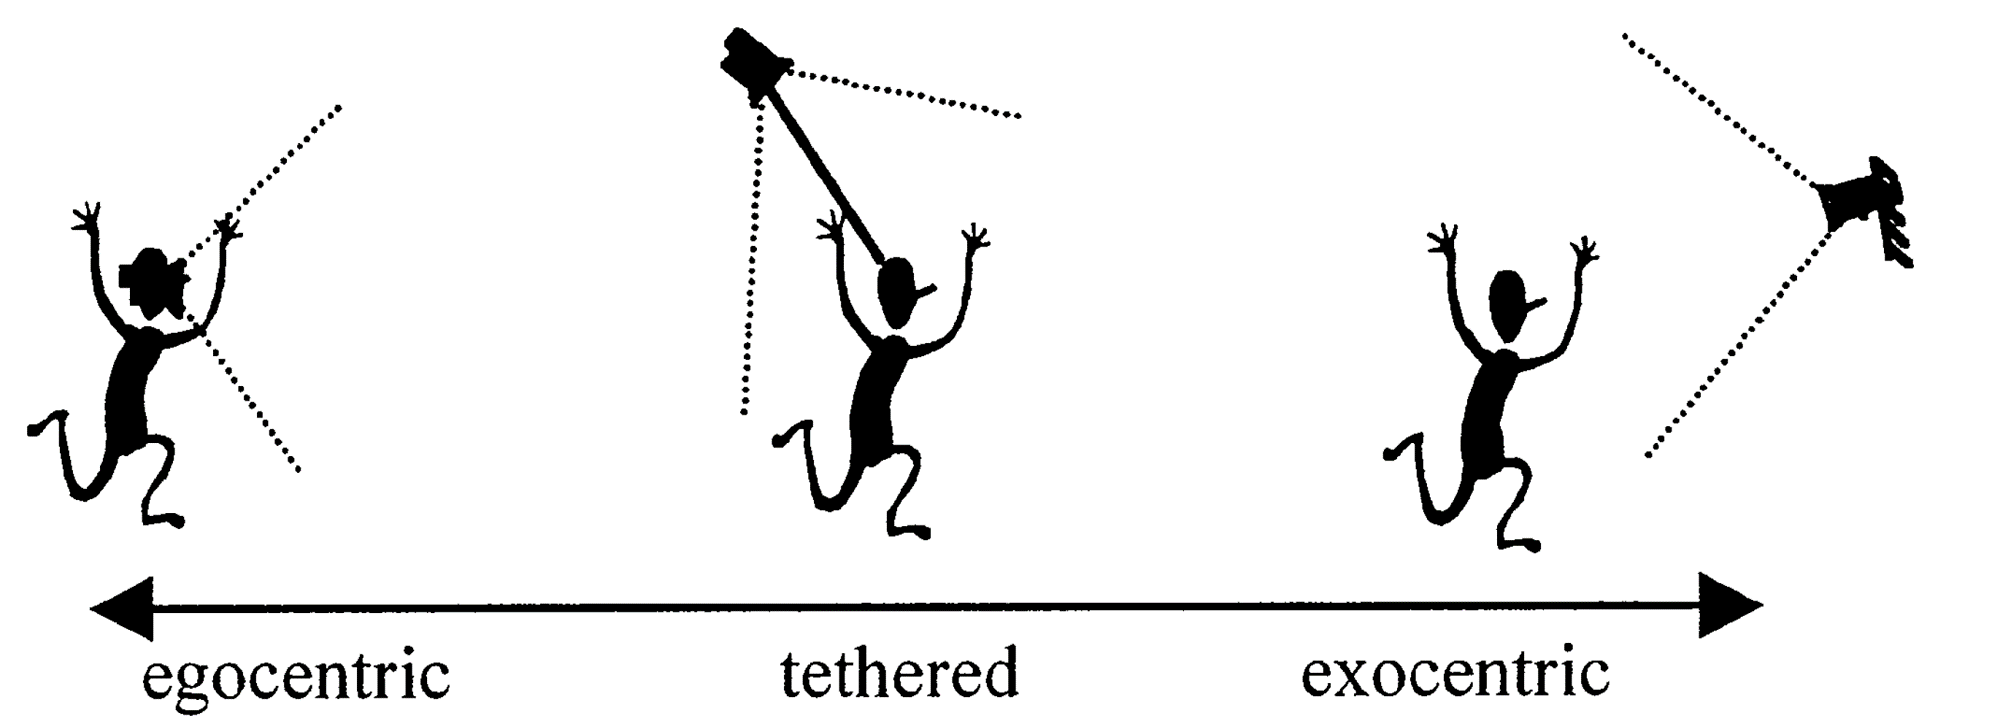
\includegraphics[width=\textwidth]{figures/ego_exo_continuum.PNG}
	\caption[Centricity continuum]{Centricity continuum by Wang and Milgram~\cite{centricitycontinuum}}
	\label{fig:ego-exo-continuum}
\end{figure}
Given a scenario where one learner mimics the movement of one teacher, five different visual perspectives are possible:
\begin{figure}[htb]
	\centering
	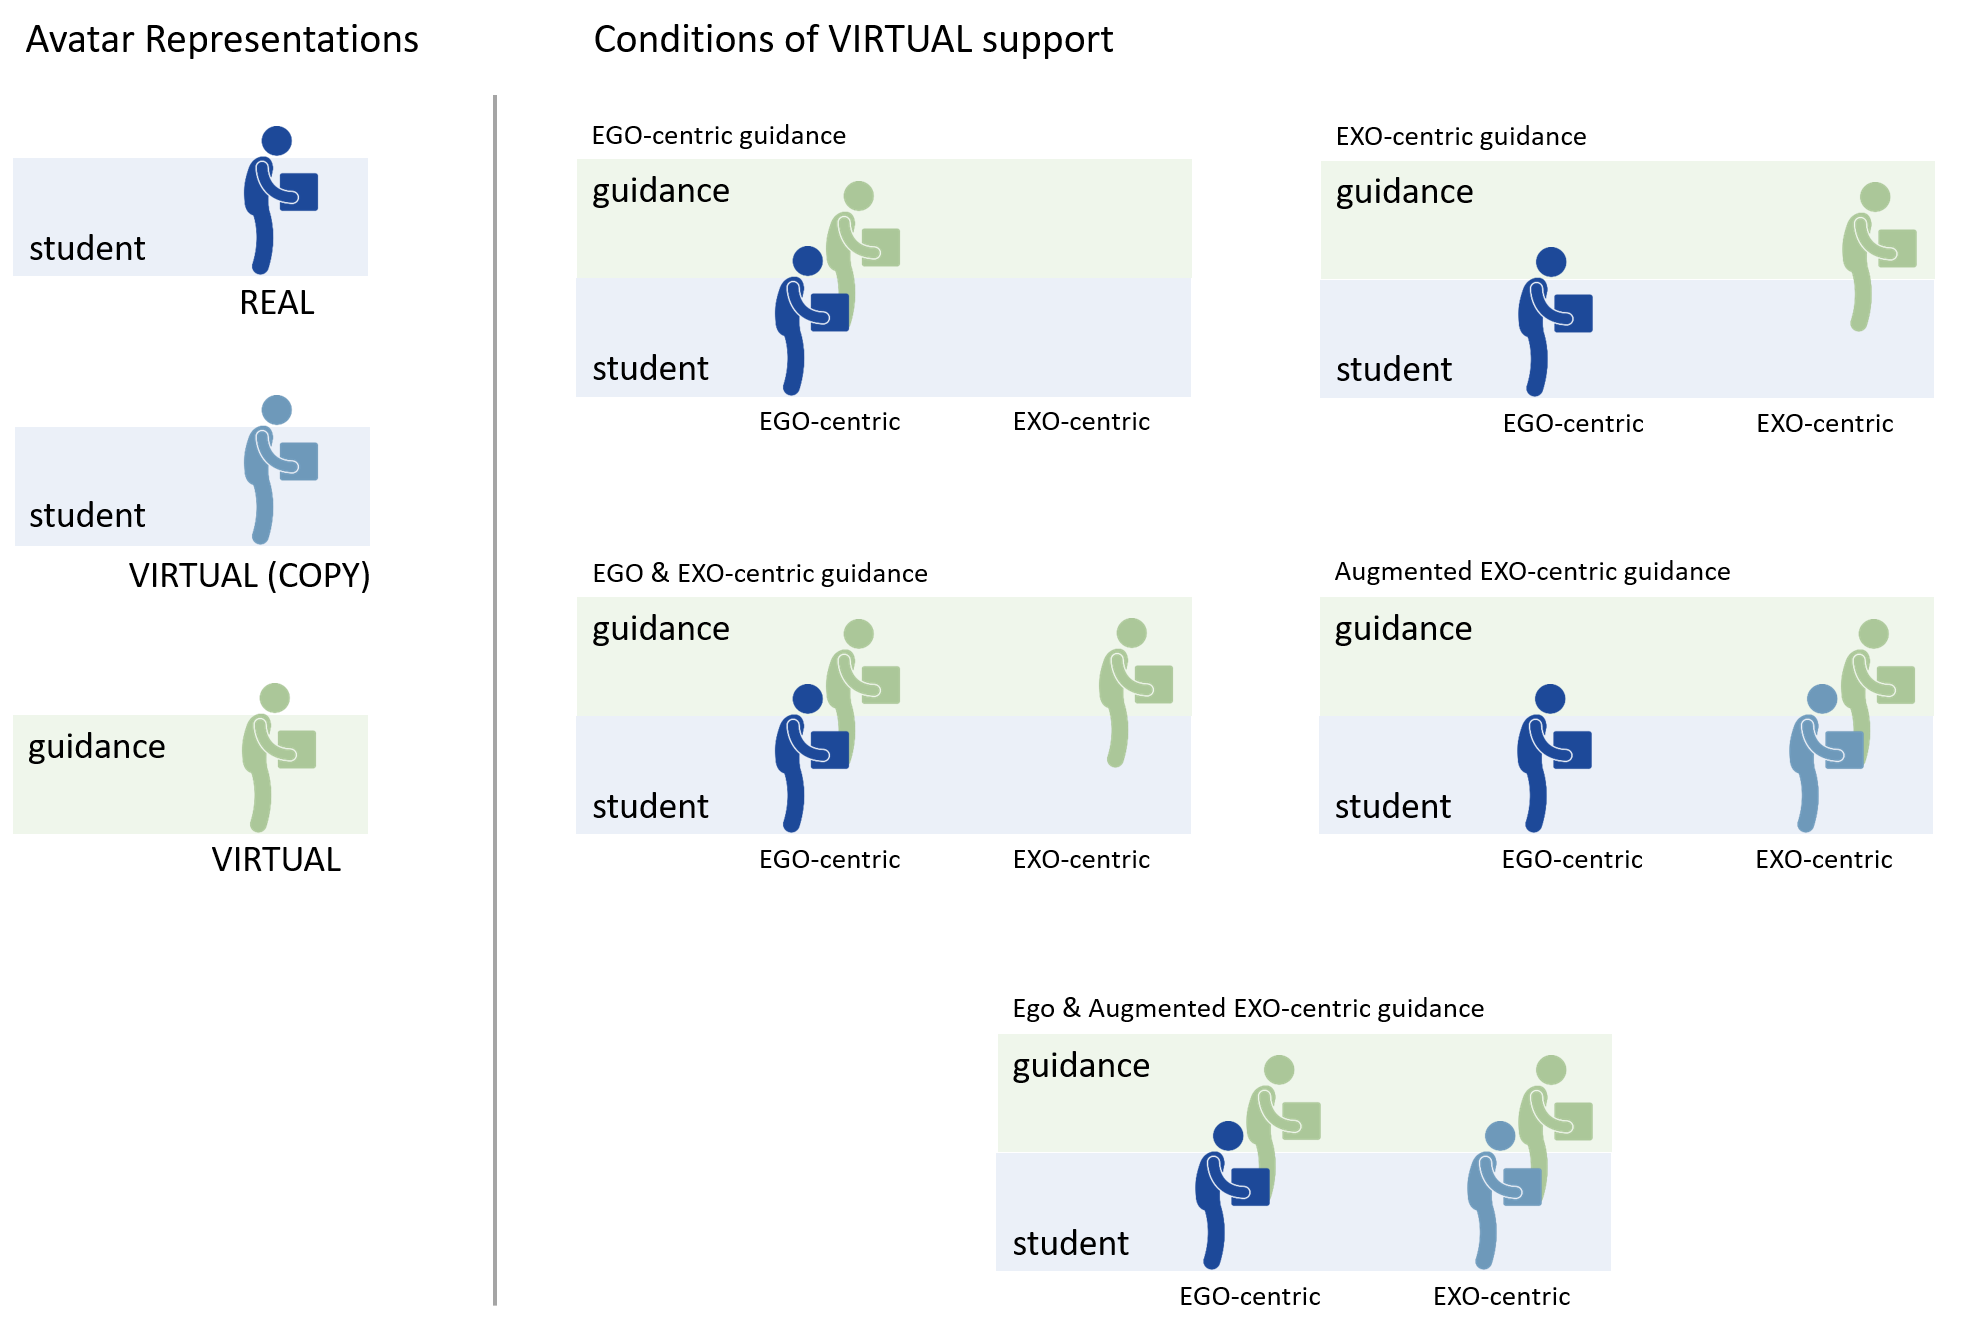
\includegraphics[width=\textwidth]{figures/perspectives.png}
	\caption[Possible perspectives]{Possible perspectives with one real world student and one real world teacher.}
	\label{fig:perspectives}
\end{figure}
\begin{itemize}
	\item Ego-centric: the avatar of the teacher is located inside the body of the avatar of the learner; the learner sees the guidance visualisation inside the own body, compare figure~\ref{fig:perspectives} top left.
	\item Exo-centric: the avatar of the guidance visualisation is located outside of the avatar of the learner; the learner sees the guidance visualisation e.g. in front of him/her, compare figure~\ref{fig:perspectives} top right.
	\item Ego \& exo-centric: the combination of ego-centric and exo-centric. The learner sees the guidance visualisation as well as inside and outside of the own body, compare figure~\ref{fig:perspectives} middle left.
	\item Augmented exo-centric: the guidance visualisation is located outside of the leraners avatar, additionally, a virtual copy of the student is located inside the exo-centric guidance visualisation, compare figure~\ref{fig:perspectives} middle right.
	\item Ego \& augmented exo-centric: the combination of the ego-centric visual perspective and the augmented exo-centric visual perspective; the learner sees the guidance visualisation inside the own body, as well as outside. Additionally, a virtual copy of the learner is located inside the exo-centric guidance visualisation, compare figure~\ref{fig:perspectives} bottom.	
\end{itemize}
All visual perspectives are worth an investigation and a comparable study with all five visual perspectives is desirable. Though, to reduce complexity and the number of participants\footnote{Due to COVID-19 pandemic}, this work will focus on three visual perspectives: ego-centric, augmented exo-centric and ego \& augmented exocentric for the following reasons. In the ego-centric visual perspective, the learner sees the teacher inside the own body. Here, the learner can see the relation of the own body to the teachers body directly. In the exo-centric visual perspective this relation cannot be seen. Thereby, the position of the learner in relation to the guidance visualisation must be guessed. That, in turn, makes the application of the speed machanic which is necessary for ego-centric guidance - described in the next section - not possible. A mechanic that is used in all conditions but one could lead to biased data, compare table~\ref{tab:mechanics}.
\begin{table}[htb]
	\centering
	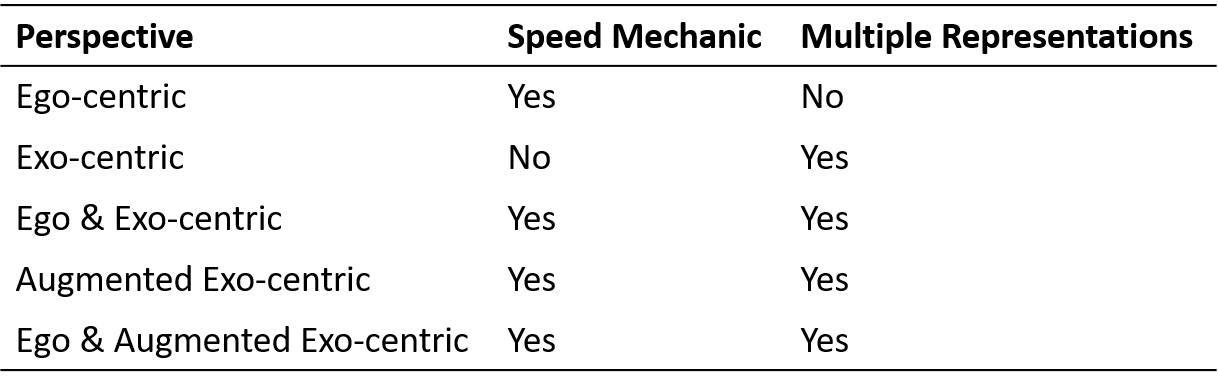
\includegraphics[width=\textwidth]{figures/mechanics_comparison.png}
	\caption[mechanics comparison]{mechanics comparison}
	\label{tab:mechanics}
\end{table}
The mechanic of multiple representations does not influence the validity of the study, because the mechanic would solve an issue that does not exist in the ego-centric perspectives.\\
In the augmented exo-centric perspective, a virtual copy of the learner is located inside the exo-centric guidance visualisation. The copy lets the learner see the relation of the own body to the guidance visualisation. Furthermore, augmenting the exo-centric guidance visualisation with the learner is applied and evaluated in related work~\cite{YouMove,thaichichua}. 
Because the speed machanic cannot be applied and the method of augmenting exo-centric guidance visualisation with a virtual copy of the learner, the augmented exo-centric perspective will be used in the proposed study. For simplicity reasons, the augmented exo-centric visual perspective will be further called exo-centric visual perspective.\\
The third visual perspective that will be used in the proposed study design is the combination of the ego-centric and exo-centric visual perspective: augmented exo-centric visual perspective, which will be further called ego \& exo-centric visual perspective.\\

\subsection{Mechanics for Motor Learning in Virtual Reality}
For teaching movments in Virtual Reality, in the exo-centric visual perspective the following issue arises. The guidance visualisation can move out of the field of view of the learner by the movement itself. Szenario: the learner and the guidance visualisation stand side-by-side, the learner sees the guidance visualisation on the left of hin/her. The guidance visualisation now indicates a movement to turn by 90 degrees to the right. When the learner follow thsi movement, the guidance visualisation will be located behind the learner after the movement ended. A guidance visualisation standing behind the learner cannot be seen by the learner.\\
This issue is solved in existing work with either the restriction of movements~\cite{freethrowsimulator,elearningma} or multiple representations of the guidance visualisation arround the learner~\cite{thaichichua,mythaichicoaches}. The restriction of movements has an strong influence in the task design and is therefore not desirable for the study proposed in this thesis, consequential for exo-centric visual perspectives multiple representations fo the guidance visualisations on strategic positions arround the learner are used.\\
In the ego-centric visual perspective, another issue araises during the teaching of transitional movements in space: walking. To understand this issue, two aspects have to be clear before. (1) The nature of an ego-centric guidance visualisation is to be located inside the learner at any time. (2) A guidance visualisation indicates movements by moving itself. If the guidance visualisatoin is about to indicate a movement away from the learner, the guidance visualisation is moving out of the students body. But a guidance visualisation that is outside of the learners body is no longer ego-centric.\\
A possible soltuion can give the centricity continuum by Wang and Milgram~\ref{fig:ego-exo-continuum}. Following the nature of the centricity continuum, the tethering distance can be increased by a small ammount and the visual perspective can still be classified as ego-centric. But now araises the question, of how far the tethering distance can be increased, with which the perspective still feels ego-centric, but the indication of the movement is considerable. For simplicity reasons, this distance is further called ego-centric tethering distance (ETD). To determine a reasonable ETD, a small formative study was conducted\footnote{A larger study was not possible because of the COVID-19 pandemic}. During this study, a non biased\footnote{The person had no prior knowledge about the system or motor learning.} person was asked to follow movements in the ego-centric visual perspective. The first movement was conducted with an ETD of 5cm. For the folowing movements the ETD was increased by 5cm each. The subjective assesment of the participant and my observations yielded best for an ETD between 15cm and 30cm. These two values are further called:
\begin{itemize}
	\item[] $ETD_{min}=15cm$
	\item[] $ETD_{max}=30cm$
\end{itemize}
Based on $ETD_{min}$ and  $ETD_{max}$ the speed mechanic is developed. The speed mechanic controls the speed of the playback of the guidance visualisation. At $ETD_{min}$ the animation plays at normal speed, at $ETD_{max}$ the guidance visualisation stops. Between $ETD_{min}$ and $ETD_{max}$ the animation speed of the guidance visualisation is linearly interpolated, compare figure~\ref{fig:speed_mechanic}.
\begin{figure}[htb]
	\centering
	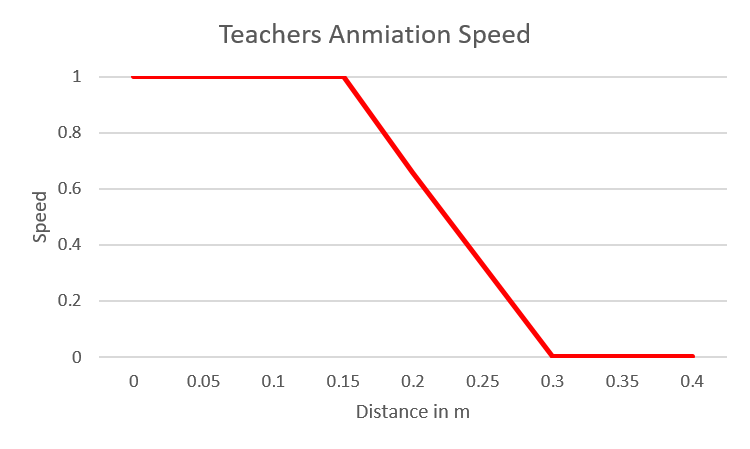
\includegraphics[width=\textwidth]{figures/speed_mechanic_chart.png}
	\caption[speed mechanic chart]{speed mechanic chart}
	\label{fig:speed_mechanic}
\end{figure}
The speed mechanic was evaluated by one\footnote{Different person than the initial. This person had no prior knowledge about the system or motor learning. Larger evaluation not possible because of COVID-19 pandemic.} person. The participant followed the guidance visualisation in the ego-centric visual perspective. Observations showed that the participant could follow the movement at ease. The opinion of the participant about the speed mechanic was very positive.


\section{Handling Physical Load}
\label{handlingphysicalload}
The handling of physical load is composed of five elemental tasks: lift, lower, push, pull and hold~\cite{mmh}. Additionally, there are non-elemental tasks like turning and sliding, ibid.. This work will use a study tasks that include the handling of physical load. Evidently, the task should consist of these elemental tasks. A tasks which consists out of the elemental tasks can be generalised to other tasks, to certain degree. To gain a strong data basis, multiple elemental tasks can be chained together (so called Unit-Combined-MMH ibid.). The task design for the proposed study founds on this basis and additionally should have a reference to real-world tasks. For the task, a simple box serves as physical load, compare chapter \todo{3}.\\
The real world provides a variety tasks that include the handling of physical load. For example in a pacel transhipment point, wearhouse workers, grinders or people that work at test stands. They pic up physical load, carry, turn and pull it. To imitate such a task, additional artifacts were created to be used in the proposed study. A table for push and pull, that could be interpreted as a machine or sorting platform and a plate on the floor that could depict for example a scale. Between the table and the scale the box can be carried. The box can be lowered and lifted from and to the scale.\\
As described in chapter \todo{4}, the legs during push and pull are in the same position if executed ergonomically. To gain variation, which is necessary to get insight how the learner can see the feet of the guidance visualisation, two non-elemental tasks were introduced: turn and fold. During this task the foot placement is different to push and pull. With the sub-tasks lift, lower, push, pull, carry, turn and fold the first task was designed. It consisted out of 28 sub-tasks were every sub-task occured 4 times. During the design of the task became clear that an additional element had to be introduced: walking. This enables more variation in the task. For example, the task executer stands at the left side of the table and pushes the box away. Now the executor can walk to the left side and pull the box.


Lift and lower can be realised by lifting the box from the floor and lower the box to the floor. For push and pull, another artifact is necessary: a table makes the execution of push and pull easier than on the ground.


manual material handling~\cite{mmh}, single: lift lower push pull carry hold, hold out because of confusion with speed mechanic, introduced carry because of variaation and flexibility in task. unit/combined mmh tasks classification.\\
baua classification?
%https://www.baua.de/EN/Topics/Work-design/Physical-workload/Types-of-workload/Types-of-workload_node.html https://www.baua.de/DE/Themen/Arbeitsgestaltung-im-Betrieb/Gefaehrdungsbeurteilung/Expertenwissen/Physische-Belastung/Heben-Halten-Tragen/Heben-Halten-Tragen_node.html



\section{Related Work: Motor Learning in Virtual Reality}
\label{section:related_work}
Training movements in Virtual Reality was investigated previously in several works. The preceeding seminar thesis (see chapter 3) provided an overview over 23 (compare table~\ref{tab:rw_overview}) of these works and evaluated six of them in detail: Tai Chi Trainer by Chua et al.~\cite{thaichichua}, YouMove by Anderson et al.~\cite{YouMove}, VR Dance Trainer by Chan et al.~\cite{vrdancetrainer}, OneBody by Hoang et al.~\cite{onebody}, LightGuide by Sodhi et al.~\cite{lightguide} and Pyhsio@Home by Tang et al.~\cite{physioathome}. Special attention was payed to the visual perspective, task, guidance visualisation and their independent and dependent variables they used in their investigations. Finnaly, the results were compared and the results of their works. An overview is depicted in table~\ref{tab:rw_overview_detail}. This work is informed by these works in various aspects. Chua et al. used the ego \& augmented exo-centric visual perspective, Hoang et al. and Sodhi et al. the ego-centric visual perspective. These visual perspectives prooved to be suited for the evaluation of motor learning in VR and is adopted for the proposed study design, compare section~\ref{section:visual_perspectives}. Furthermore, Chan et al. and Chua et al. used high realisitc avatars as guidance visualisation, which are used in the proposed study design, compare seminar thesis chapter 3.3. Furthermore, recent research indicates, that high realism avatars outperforms abstract avatars~\cite{max,perspectivematters} All authors used a performance measure to evaluate the performend movements of the participants of their studies. Especially the distance based measures informed the measures used in the proposed study design, compare~\ref{section:measures_for_ml}.\\
The relatively new technology of Vive Trackers in combination with inverse Kinematics (see project report chapter 2.1 and 2.2) is not used by the above mentioned works. Sra et al.~\cite{samesetup} used this technology in 2018 for their system Your Place and Mine to render human shaped avatars.\\
The results of related work yielded in no clear conclusion about the influence of the perspectives on motor learning. Chua et al. found no difference in the performance between the visual perspectives, Anderson et al. and Chan et al. found out that their exo-centric visual perspectives in Virtual Reality outperforms traditional video guidance. The works of Hoang et al. and Sodhi et al. conclude that the ego-centric perspective outperforms the exo-centric visual perspective. But an investigation of how the visual perspective influences motor learning was not investigated. Recently, in December 2020, Yu et al.~\cite{perspectivematters} conducted three independent studies to close this gap. In the first study Yu et al. compared the ego-centric visual perspective and a 2D-mirror for single arm movements. In the second study they compared the ego-centric and exo-centric visual perspective for Yoga. In the third study they compared the ego-centric visual perspective with an 3D-mirror for arm movements. Yu et al. conclude their findings in a design guideline for systems training Motor Learning in Virtual Reality: use the ego-centric visual perspective if the type of motion allows, consider alternatives for other types of motions, ibidem. In all three studies the ego-centric visual perspective outperformed the other perspectives, if the movement was clearly visible from the ego-centric visual perspective. This work, in contrast, focus on full body movements that include the handling of physical load. Furthermore, this work provides a third visual perspective where the ego-centric and exo-centric visual perspective is combined.
\begin{table}[htb]
	\centering
	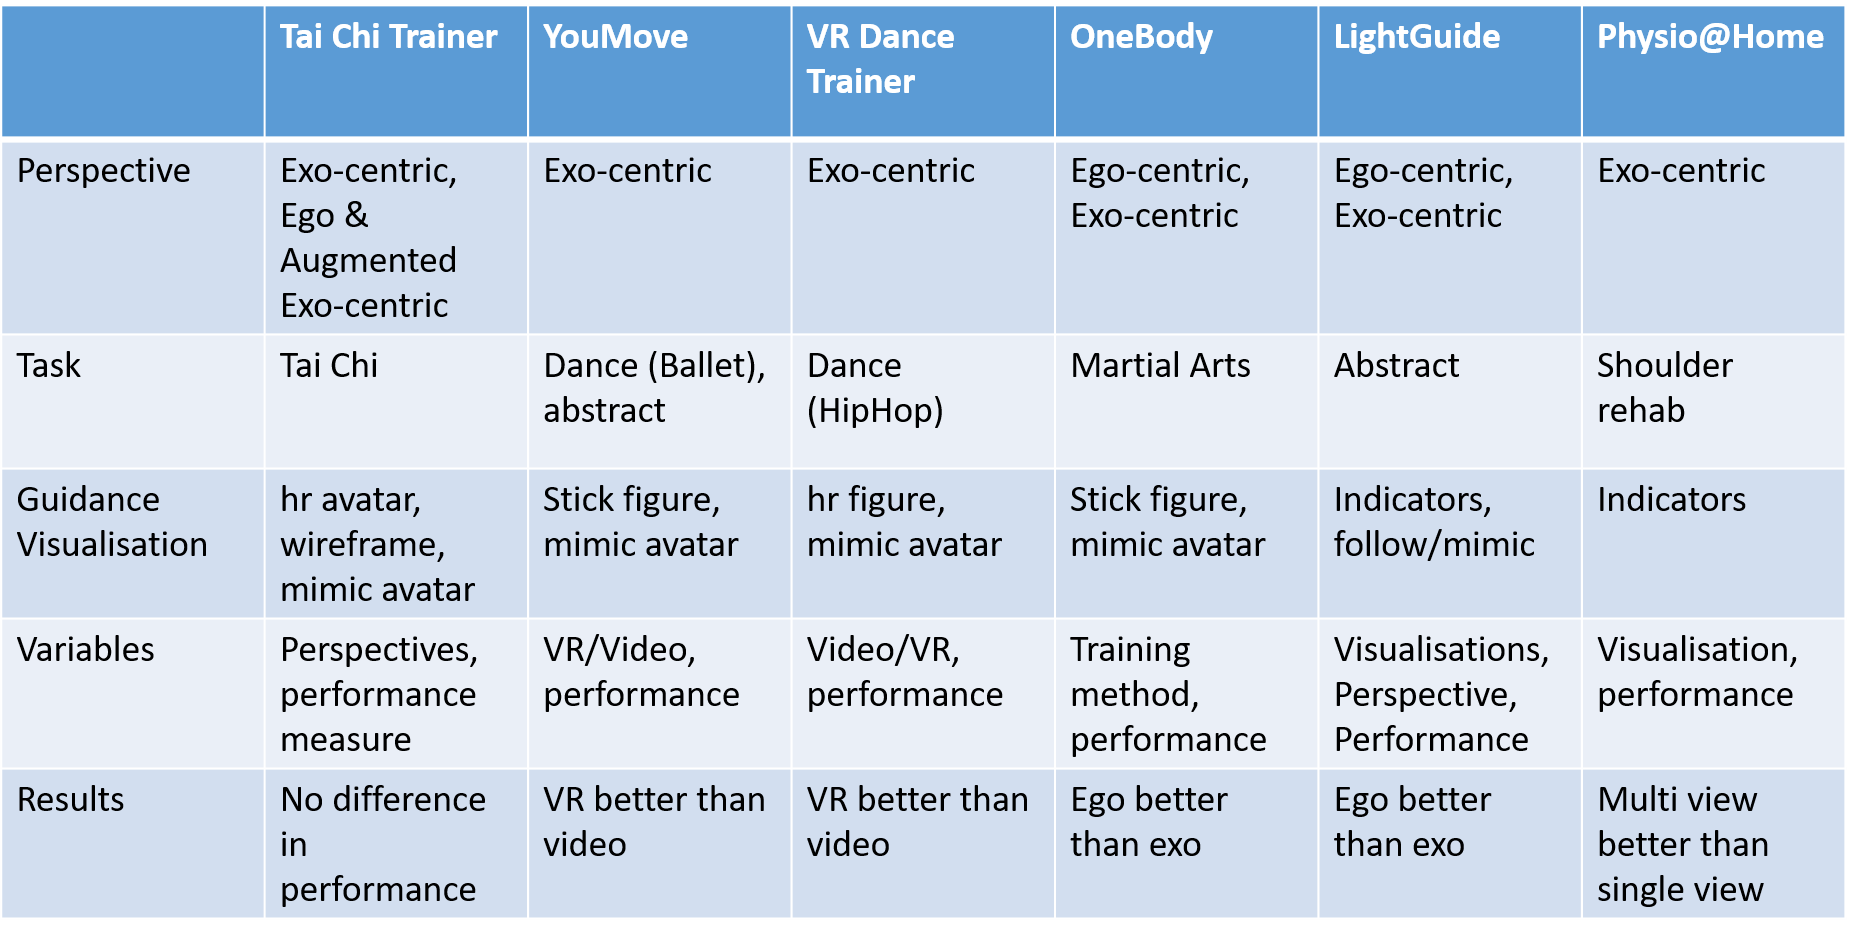
\includegraphics[width=\textwidth]{figures/detail_paper_overview.png}
	\caption[Overview seminar evaluation]{Overview seminar evaluation}
	\label{tab:rw_overview_detail}
\end{table}

\begin{table}[htb]
	\centering
	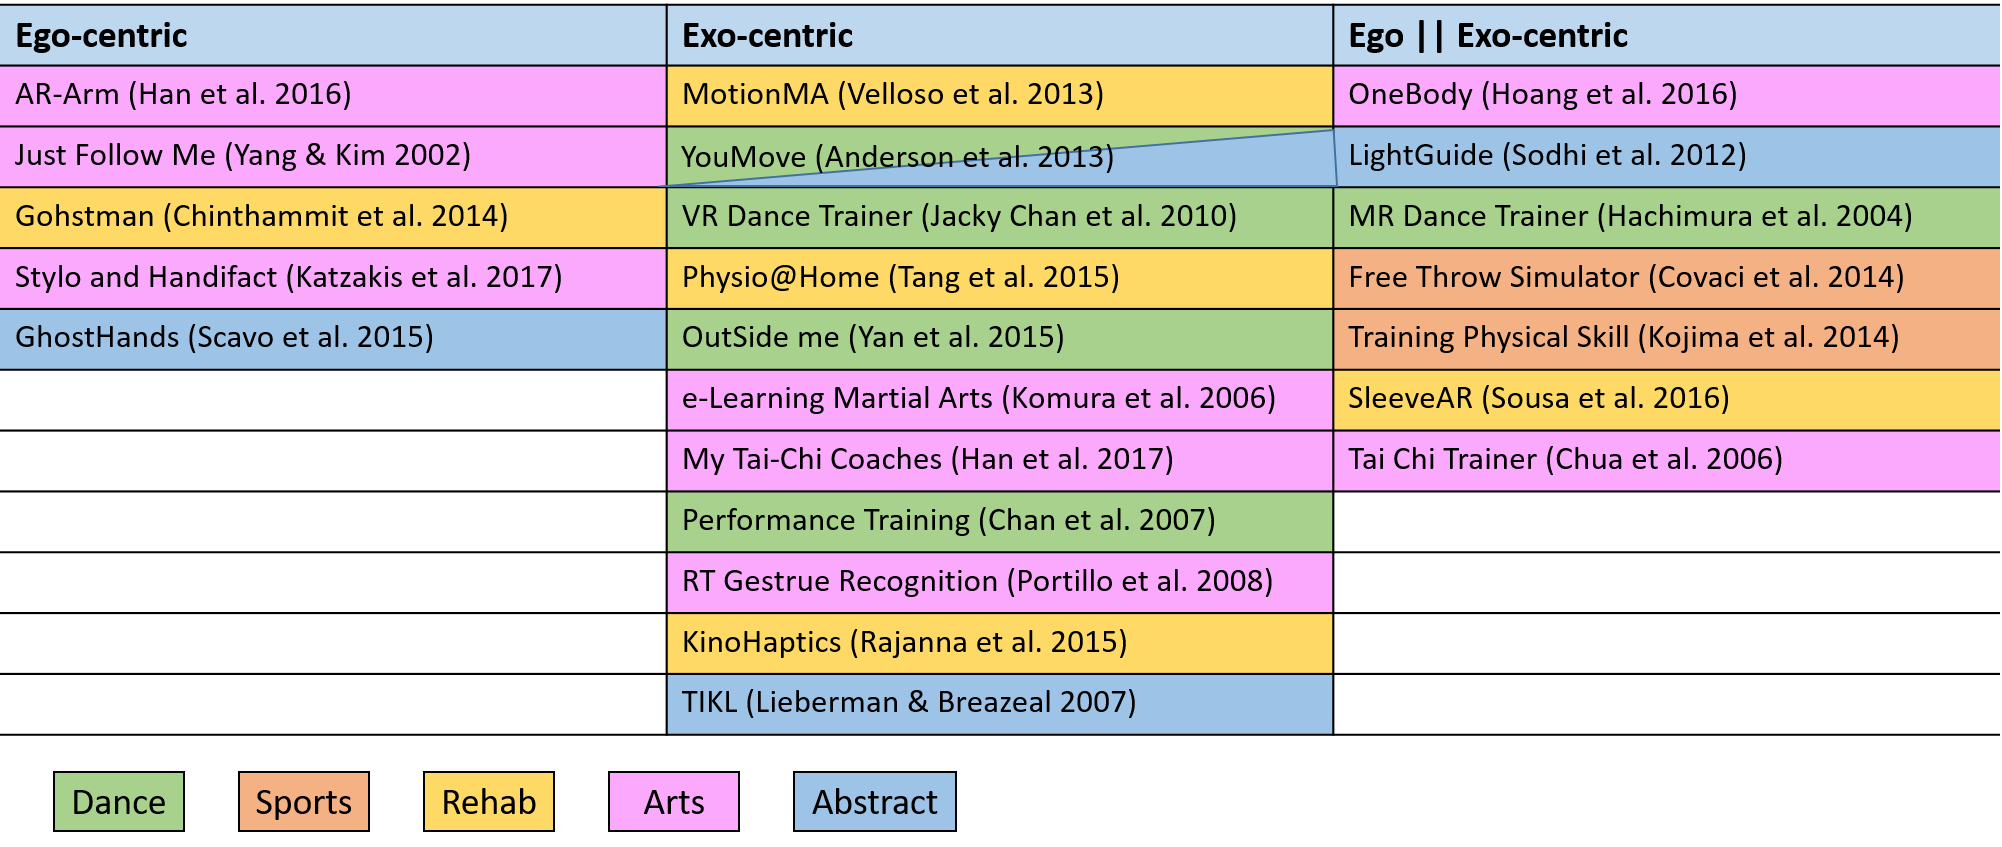
\includegraphics[width=\textwidth]{figures/rw_overview.png}
	\caption[Overview seminar evaluation]{Overview Related Work divided by perspective and task}
	\label{tab:rw_overview}
\end{table}
\section{Research Contribution Statement}
\label{delimination_contribution}
The conduction of the proposed study will produce data that serves as a reasonable basis for designers of VR Motor Learning systems.
bekannte arbeiten und deren ergebnisse über motor learning in VR\\
\\
auf basis dieses kapitels wird die studie geformt

